\documentclass[parskip=full]{scrartcl}
\usepackage[top=2.54cm, bottom=2.54cm, left=2.54cm, right=2.54cm]{geometry}
\usepackage[utf8]{inputenc} % use utf8 file encoding for TeX sources
\usepackage[T1]{fontenc}    % avoid garbled Unicode text in pdf
\usepackage[ngerman]{babel}  % german hyphenation, quotes, etc
\usepackage{hyperref}       % hyperlinks in document
\usepackage{glossaries}     % glossary 
\usepackage{enumerate}      % advanced enumeration
\usepackage[shortlabels]{enumitem}
\usepackage[dvipsnames]{xcolor}
\usepackage{graphicx}
\usepackage{caption}        % add captions
\usepackage{adjustbox}      % add adjustmentbox
\usepackage{csquotes}

% Set footer and header bar
\usepackage[headsepline, footsepline]{scrlayer-scrpage}
\addtokomafont{headsepline}{\color{BlueViolet}}
\addtokomafont{footsepline}{\color{BlueViolet}}
\KOMAoptions{headsepline=1.25pt:\textwidth}
\KOMAoptions{footsepline=1.25pt:\textwidth}
\clearpairofpagestyles
\rofoot{\thepage}
\ihead{Write your own Android App: SpiceSquad}

% set the hyperlink style in the document
\hypersetup{
    pdftitle={PSE: Entwurfsheft},
    pdfborderstyle={/S/U/W 1},
    colorlinks,
    linkcolor={black!50!black},
    citecolor={blue!50!black},
    urlcolor={blue!80!black}
}

% sets right quotation for "
\MakeOuterQuote{"}

%change figure numbering
\renewcommand{\thefigure}{\thesection.\arabic{figure}}

%add command to hide subsections from toc
\newcommand{\changelocaltocdepth}[1]{%
  \addtocontents{toc}{\protect\setcounter{tocdepth}{#1}}%
  \setcounter{tocdepth}{#1}%
}

\newcommand{\enablesubsectionnumbering}[1]{
    \renewcommand{\thesubsection}{$\langle$#1\arabic{subsection}0$\rangle$}
    \changelocaltocdepth{1} 
}

\newcommand{\resetsubsectionnumbering}{
    \renewcommand{\thesubsection}{\arabic{section}.\arabic{subsection}}
    \changelocaltocdepth{3} 
}

% glossary
\makeglossaries
\renewcommand{\glossarysection}[2][]{}

\begin{document}
\newglossaryentry{label}{
    name=Label,
    plural=Labels,
    description={Rezepte können mit bezeichnenden Stichwörtern, sogenannten Labels, versehen werden. Dies ermöglicht das Filtern von Rezepten nach bestimmten Eigenschaften (z.B. vegetarisch, glutenfrei, halal)}
}

\begin{titlepage}
    \begin{center}
        \begin{Huge}
            {\textbf{Write your own Android App: SpiceSquad}}
        \end{Huge}
        \vspace{12px}

        Praxis der Softwareentwicklung (PSE)\\
        Sommersemester 2023\\
        \vspace{150px}

        \begin{Huge}
            {\textbf{Entwurfsheft}}
        \end{Huge}
        \vspace{12px}

        \textbf{Auftraggeber}\\
        Karlsruher Institut für Technologie\\
        KASTEL — Institut für Informationssicherheit und Verlässlichkeit\\
        \vspace{330px}

        \textbf{Auftragnehmer}\\
        Karlsruher Intellektuelle\\
        Henri Becker, Konrad Knappe, Lukas Schwarz, Raphael Zipperer\\
    \end{center}
\end{titlepage}

\tableofcontents
\newpage

\section*{Gender-Hinweis}
Zur besseren Lesbarkeit wird in diesem Entwurfsheft das generische Maskulinum verwendet.
Die in diesem Heft verwendeten Personenbezeichnungen beziehen sich – sofern nicht anders kenntlich gemacht – auf alle Geschlechter.


\section{Presentation layer}
    %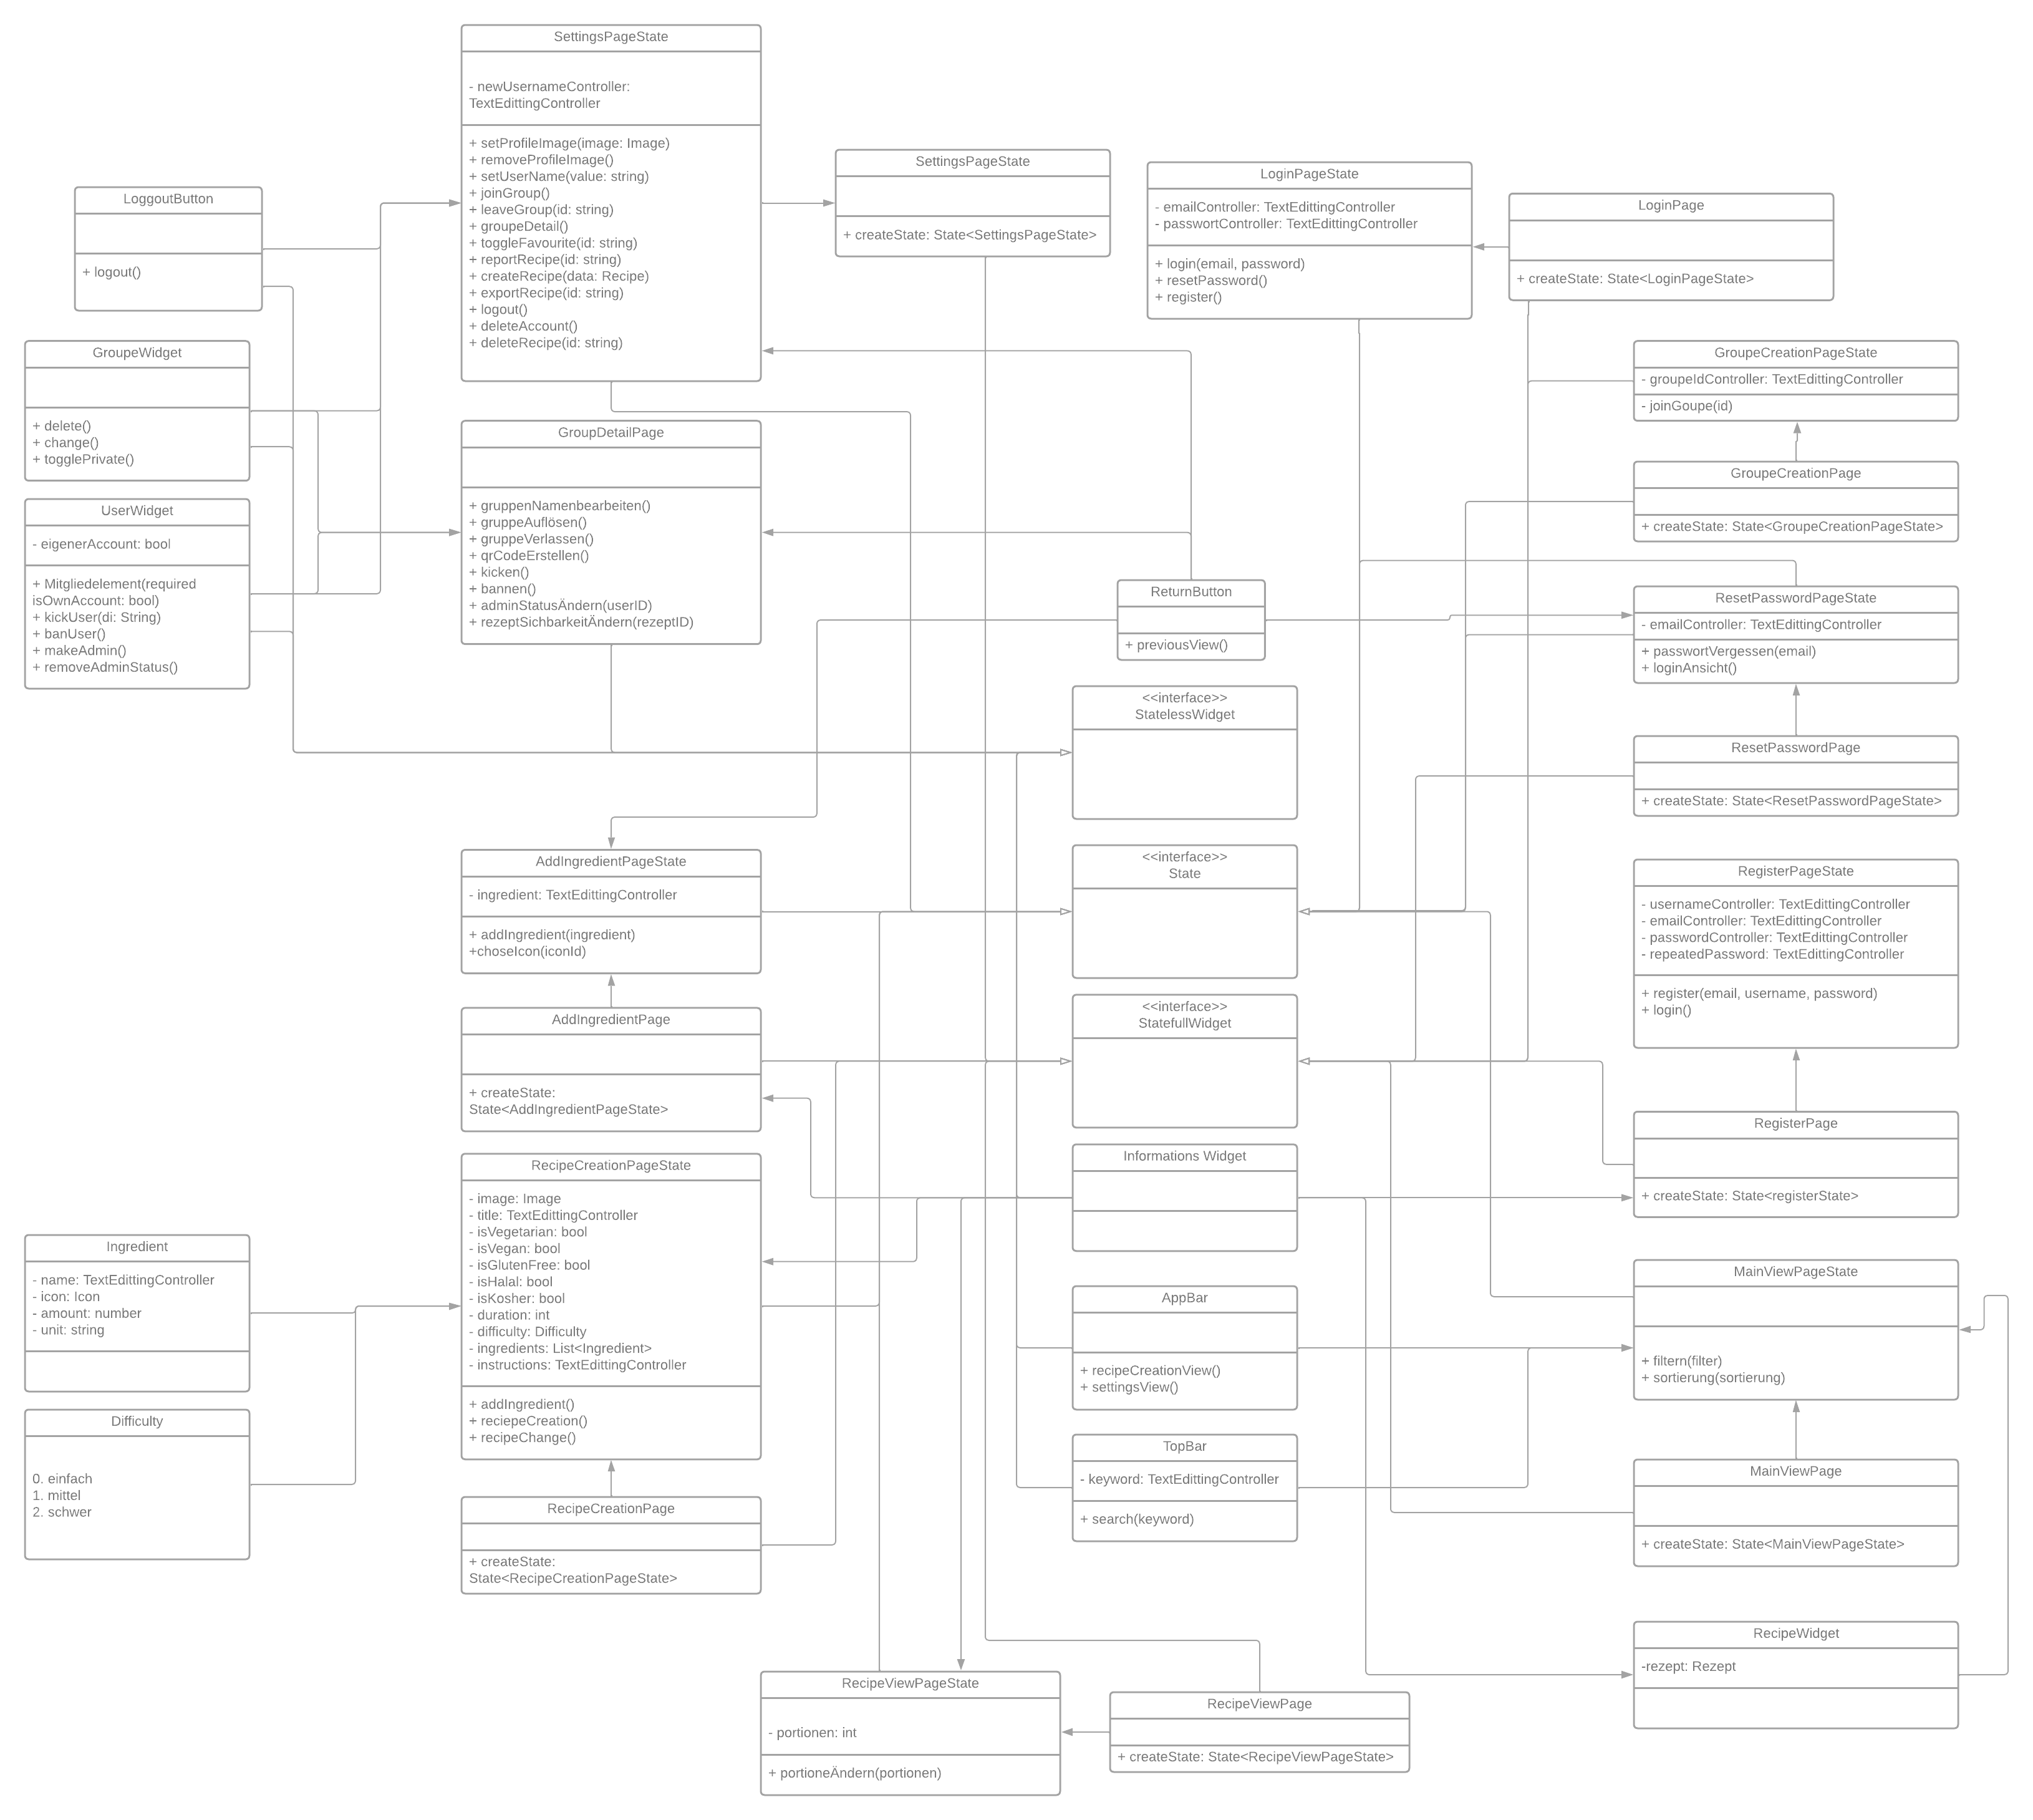
\includegraphics[width = 180mm]{entwurfsheft/images/Presentation-layer/Presentation-Layer.png}
    \newpage
    \subsection{Recipe Creation Page}
        Die Klassen beinhaltet alle nötigen Funktionen und Attribute um die Rezept-Erstell-Ansicht darzustellen.\newline
        \textbf{Attributes}
        \begin{itemize}
            \item image: Hochgeladenes Bild welches den anderen Nutzern in der Rezeptansicht angezeigt werden soll.
            \item title: Die eingegebene Zeichenkette für den Titel des Rezepts.
            \item isVegetarian: Der vom Nutzer angegebene Boolean ob das \gls{label} Vegetarisch dem Leser angezeigt werden soll.
            \item isVegan: Der vom Nutzer angegebene Boolean ob das \gls{label} Vegan dem Leser angezeigt werden soll.
            \item isGlutenFree: Der vom Nutzer angegebene Boolean ob das \gls{label} Glutenfrei dem Leser angezeigt werden soll.
            \item isHalal: Der vom Nutzer angegebene Boolean ob das \gls{label} Halal dem Leser angezeigt werden soll.
            \item isKosher: Der vom Nutzer angegebene Boolean ob das \gls{label} Koscher dem Leser angezeigt werden soll.
            \item duration: Die vom Nutzer eingegebene Ganzzahl, welche die Zubereitunszeit in Minuten angibt.
            \item dificullty: Die vom Nutzer ausgewählte \gls{schwierigkeit} des Rezepts
            \item ingerdients: Eine Liste an Ingerdients, welche in der AddIngredientPage erstellt wurde:
            \item instructions: Die vom Nutzer angegeben Zeichenkette für die Beschreibung des Rezepts.
        \end{itemize}
        
        \textbf{Methods}
        \begin{itemize}
            \item addIngredient(): Die Page AddIngredientPage wird aufgerufen.
            \item recipeSave(): Die Methode ruft, abhängig davon ob das Rezept neu erstellt wird oder nur verändert wurde, entweder recipeCreation() oder recipeChange() auf.
        \end{itemize}

        
        %\begin{figure}[htp]
        %    \begin{minipage}
        %        [t]{0.49\textwidth}
        %        \centering
        %        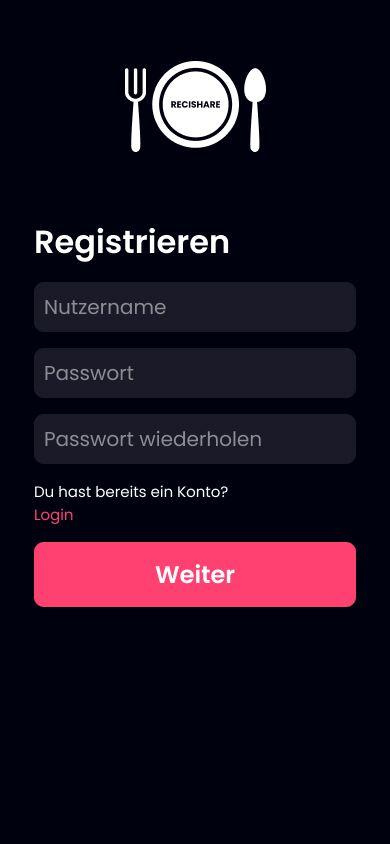
\includegraphics[height=80mm]{pflichtenheft/images/benutzeroberfläche/RegisterView.jpg}
        %        \caption{Registrierungsansicht}
        %    \end{minipage}
        %    \begin{minipage}
        %        [t]{0.49\textwidth}
        %        \centering
        %        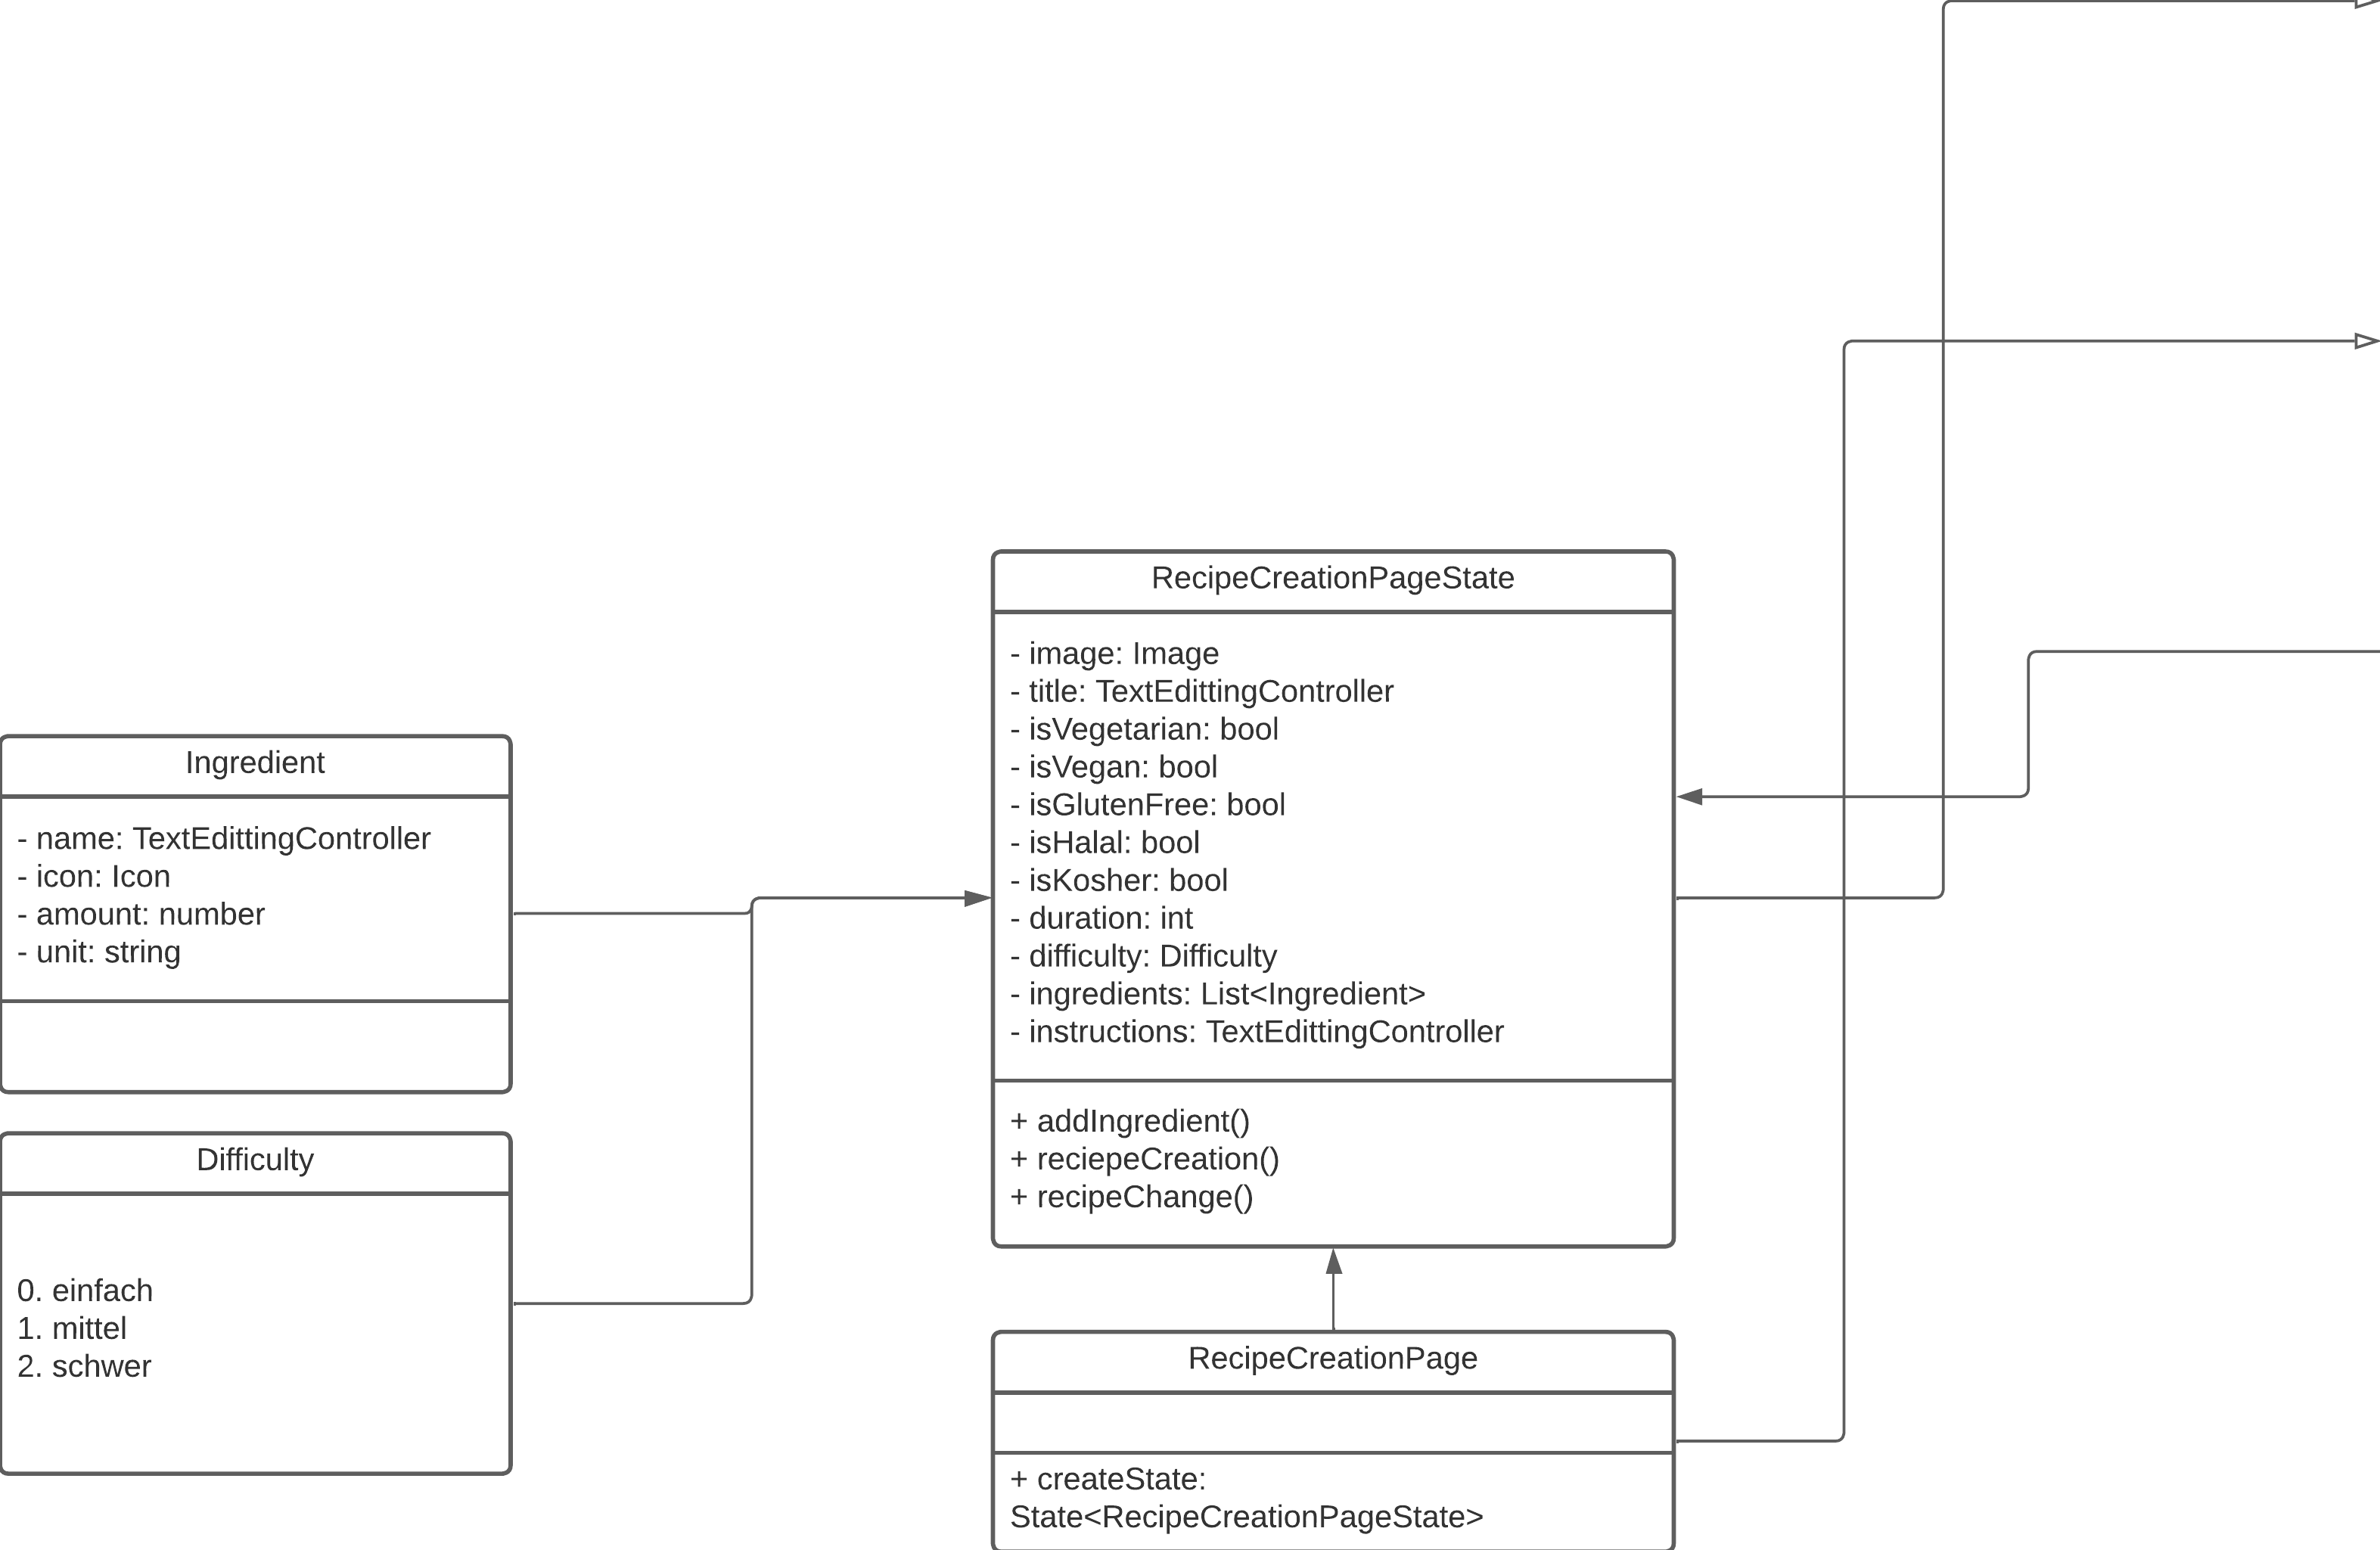
\includegraphics[height = 50mm]{entwurfsheft/images/Presentation-layer/Recipe Creation Page.png}
        %        \caption{RecipeCreationPage}
        %    \end{minipage}
        %\end{figure}

 
\newpage

\section{Datenbank}
Die zugrundeliegende Datenbank soll möglichst nah an unseren Entitäten orientiert sein, um inkonsistente Daten zu vermeiden. Daher wird für das Projekt die Datenbank "PostgreSQL" verwendet. Sie unterstützt relationale Datenformate und ist daher optimal für unsere Anforderungen geeignet. Zudem ist sie Open-Source und kostenlos und erfreut sich seit 35 Jahren großer Beliebtheit.
\subsection{Datenbankschema}
\begin{figure}[htp]
    \centering
    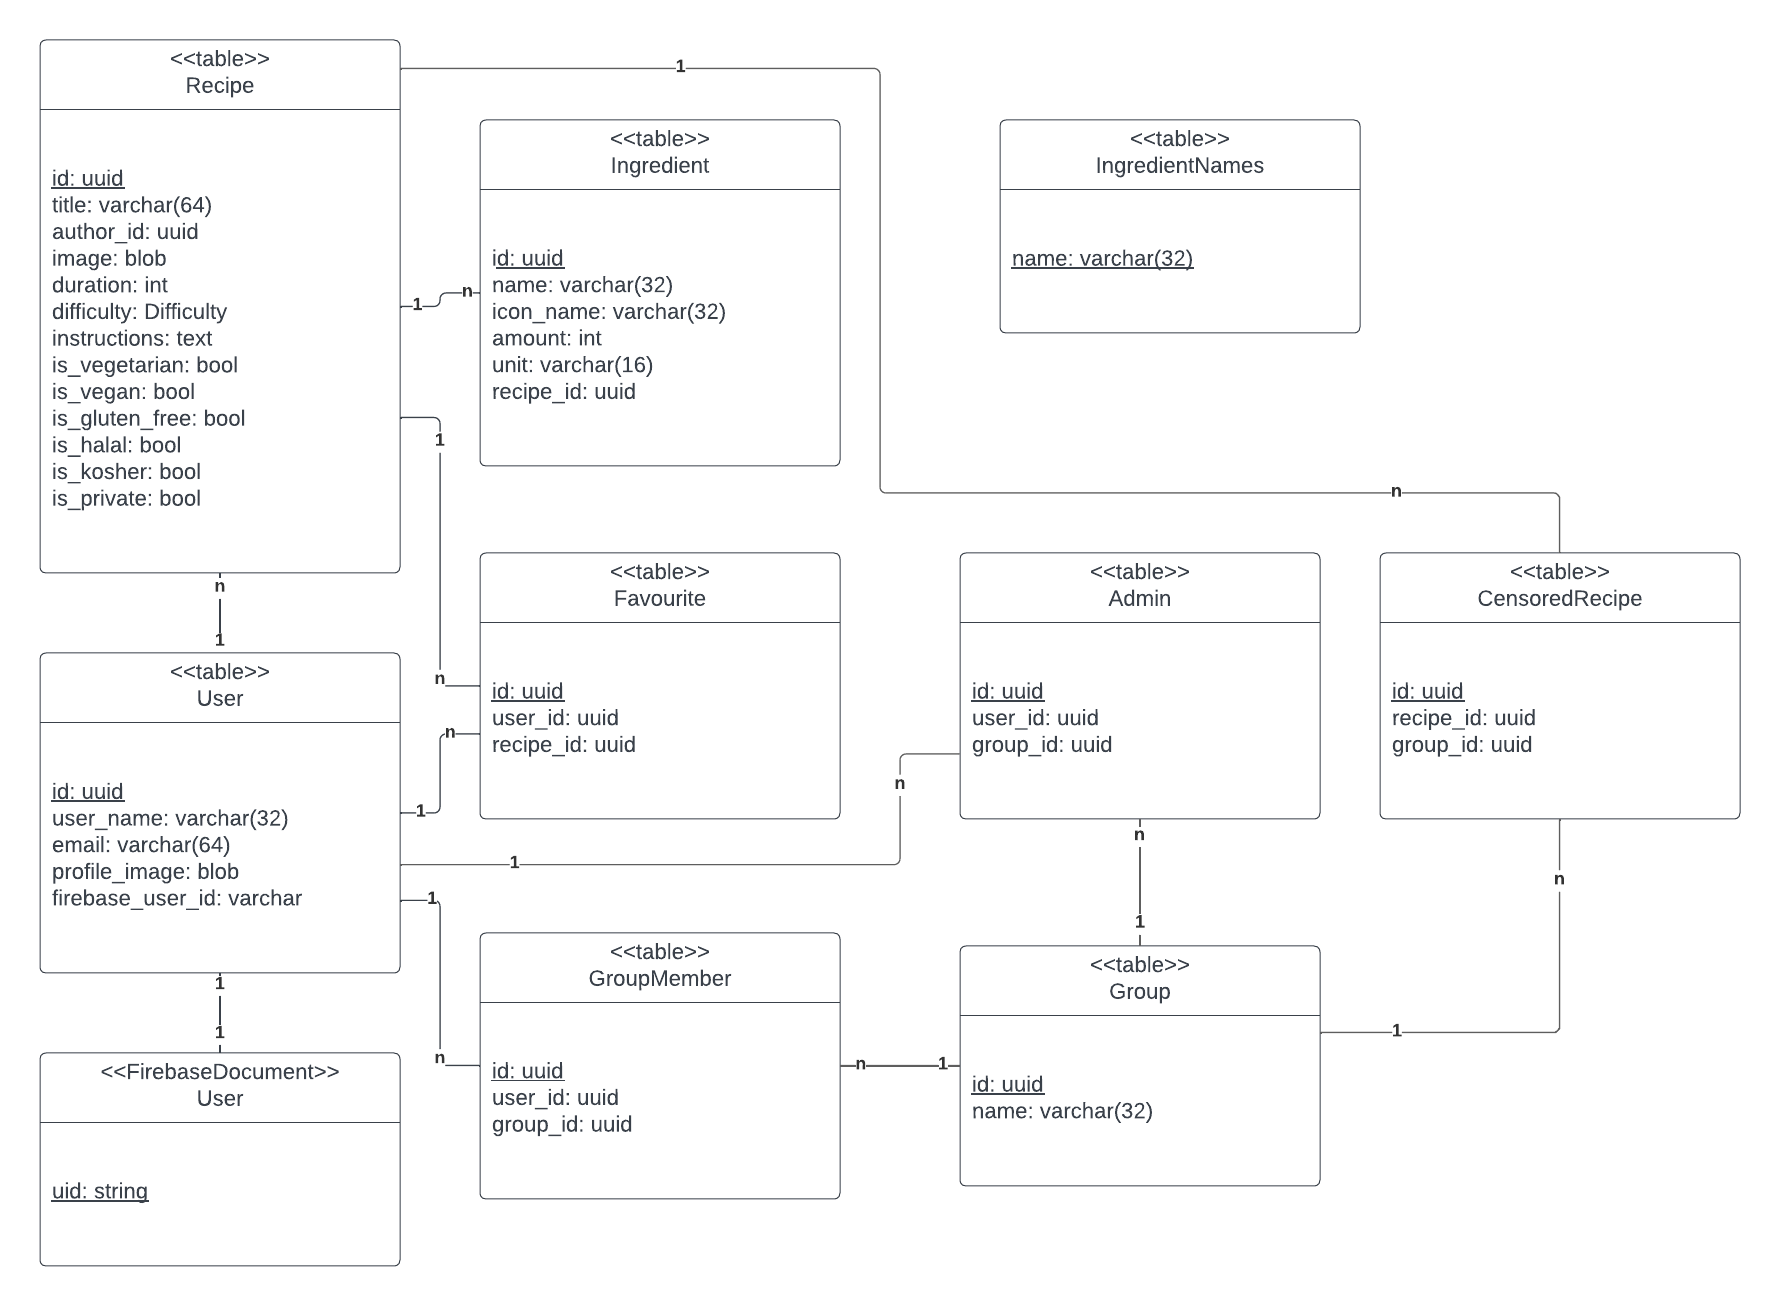
\includegraphics[width = \linewidth]{images/Database/schema.png}
    \caption{Datenbankschema}
\end{figure}
Im Datenbankschema werden die einzelnen Entitäten der App abgebildet. Die einzelnen Tabellen werden nun genauer erläutert.
\newpage
\subsubsection{Recipe}
Die Tabelle "Recipe" enthält die Rezepte und besitzt die folgenden Attribute:
\paragraph{id (uuid - primary key):} Die Id stellt den Primärschlüssel des Rezepts dar und muss daher eindeutig und nicht leer sein. Der Datentyp ist \Gls{uuid}. Sie wird automatisch generiert.
\paragraph{title (varchar(64) - not null):} Der Titel des Rezepts. Der Datentyp ist \Gls{varchar}. Er darf nicht leer und maximal 64 Zeichen lang sein.
\paragraph{author\_id (uuid - not null, foreign key):} Hierbei handelt es sich um die Id des Autors des Rezepts als Fremdschlüssel. Sie darf nicht leer sein und der Datentyp ist \Gls{uuid}, da es sich um eine Id handelt.
\paragraph{image (blob):} Das Bild des Rezepts in binär Code. Der Datentyp ist \Gls{blob}.
\paragraph{duration (int - not null):} Die Zubereitungszeit des Rezepts in Minuten. Der Datentyp ist Integer. Sie darf nicht leer sein.
\paragraph{difficulty (Difficulty - not null):} Die Schwierigkeit des Rezepts, die nicht leer sein darf. Der Datentyp "Difficulty" ist ein Enum, mit den Werten "easy", "medium" und "hard".
\paragraph{instructions (text - not null):} Die Zubereitungsanleitung des Rezepts, die nicht leer sein darf. Der Datentyp ist Text, was einer unbegrenzten Zeichenkette entspricht.
\paragraph{is\_vegetarian (bool - not null):} Gibt an, ob das \Gls{label} "Vegetarisch" aktiviert ist. Der Datentyp ist Boolean und darf nicht leer sein.
\paragraph{is\_vegan (bool - not null):} Gibt an, ob das \Gls{label} "Vegan" aktiviert ist. Der Datentyp ist Boolean und darf nicht leer sein.
\paragraph{is\_gluten\_free (bool - not null):} Gibt an, ob das \Gls{label} "Glutenfrei" aktiviert ist. Der Datentyp ist Boolean und darf nicht leer sein.
\paragraph{is\_halal (bool - not null):} Gibt an, ob das \Gls{label} "Halal" aktiviert ist. Der Datentyp ist Boolean und darf nicht leer sein.
\paragraph{is\_kosher (bool - not null):} Gibt an, ob das \Gls{label} "Koscher" aktiviert ist. Der Datentyp ist Boolean und darf nicht leer sein.
\newpage
\subsubsection{Ingredient}
Die Tabelle "Ingredient" enthält die Zutaten, die den eizelnen Rezepten zugeordnet sind und besitzt die folgenden Attribute:
\paragraph{id (uuid - primary key):} Die Id stellt den Primärschlüssel der Zutat dar und muss daher nicht leer und eindeutig sein. Der Datentyp ist \Gls{uuid}. Sie wird automatisch generiert. 
\paragraph{name (varchar(32) - not null):} Der Name der Zutat. Der Datentyp ist \Gls{varchar}. Er darf nicht leer und maximal 32 Zeichen lang sein.
\paragraph{icon\_name (varchar(32))} Der Name des Icons, das die Zutat repräsentiert. Der Datentyp ist \Gls{varchar}. Er ist maximal 32 Zeichen lang.
\paragraph{amount (int - not null):} Die Menge der Zutat in der jeweiligen Einheit. Sie darf nicht leer sein und der Datentyp ist Integer.
\paragraph{unit (varchar(16)):} Die Einheit der Zutat. Der Datentyp ist \Gls{varchar}. Sie ist maximal 16 Zeichen lang und optional. 
\paragraph{recipe\_id (uuid - not null, foreign key):} Hierbei handelt es sich um die Id des Rezepts, zu dem die Zutat gehört, als Fremdschlüssel. Sie darf nicht leer sein und der Datentyp ist \Gls{uuid}, da es sich um eine Id handelt.
\newpage
\subsubsection{IngredientNames}
Die Tabelle "IngredientNames" enthält lediglich die Namen der Zutaten, die in der Vorschlagsliste beim Zutaten erstellen angezeigt werden. Sie besitzt die folgenden Attribute:
\paragraph{name (varchar(32) - primary key):} Der Name der Zutat. Der Datentyp ist \Gls{varchar}. Es handelt sich um den Primärschlüssel und der Name muss daher eindeutig und nicht leer sein.
\newpage
\subsubsection{User}
Die Tabelle "User" enthält die Benutzer der App und besitzt die folgenden Attribute:
\paragraph{id (uuid - primary key):} Die Id stellt den Primärschlüssel des Benutzers dar und muss daher eindeutig und nicht leer sein. Der Datentyp ist \Gls{uuid}. Sie wird automatisch generiert.
\paragraph{user\_name (varchar(32) - not null):} Der Benutzername des Benutzers. Der Datentyp ist \Gls{varchar}. Er darf nicht leer und maximal 32 Zeichen lang sein.
\paragraph{email (varchar(64) - not null):} Die E-Mail-Adresse des Benutzers. Der Datentyp ist \Gls{varchar}. Sie darf nicht leer und maximal 64 Zeichen lang sein.
\paragraph{profile\_image (blob):} Das Profilbild des Benutzers in binär Code. Der Datentyp ist \Gls{blob}.
\paragraph{firebase\_user\_id (varchar - not null, unique)} Die Id des Benutzers, die in der Firebase Datenbank hinterlegt ist. Der Datentyp ist \Gls{varchar}. Sie muss eindeutig und nicht leer sein. Sie dient als Fremdschlüssel über die Datenbank hinweg zu Firebase.
\newpage
\subsubsection{Favourite}
Die Tabelle "Favourite" repräsentiert die Many-To-Many-Beziehung zwischen den Benutzern und den Rezepten, die sie favorisiert haben. Sie besitzt die folgenden Attribute:
\paragraph{id (uuid - primary key):} Die Id stellt den Primärschlüssel der Beziehung dar und muss daher eindeutig und nicht leer sein. Der Datentyp ist \Gls{uuid}. Sie wird automatisch generiert.
\paragraph{user\_id (uuid - not null, foreign key):} Hierbei handelt es sich um die Id des Benutzers, der das Rezept favorisiert hat, als Fremdschlüssel. Sie darf nicht leer sein und der Datentyp ist \Gls{uuid}, da es sich um eine Id handelt.
\paragraph{recipe\_id (uuid - not null, foreign key):} Hierbei handelt es sich um die Id des Rezepts, das favorisiert wurde, als Fremdschlüssel. Sie darf nicht leer sein und der Datentyp ist \Gls{uuid}, da es sich um eine Id handelt.
\newpage
\subsubsection{Group}
Die Tabelle "Group" enthält die Gruppen bzw. Squads und besitzt die folgenden Attribute:
\paragraph{id (uuid - primary key):} Die Id stellt den Primärschlüssel der Gruppe dar und muss daher eindeutig und nicht leer sein. Der Datentyp ist \Gls{uuid}. Sie wird automatisch generiert.
\paragraph{name (varchar(32) - not null):} Der Name der Gruppe. Der Datentyp ist \Gls{varchar}. Er darf nicht leer und maximal 32 Zeichen lang sein.
\newpage
\subsubsection{GroupMember}
Die Tabelle "GroupMember" repräsentiert die Many-To-Many-Beziehung zwischen den Gruppen und den Benutzern, die Mitglied der Gruppe sind. Sie besitzt die folgenden Attribute:
\paragraph{id (uuid - primary key):} Die Id stellt den Primärschlüssel der Beziehung dar und muss daher eindeutig und nicht leer sein. Der Datentyp ist \Gls{uuid}. Sie wird automatisch generiert.
\paragraph{user\_id (uuid - not null, foreign key):} Hierbei handelt es sich um die Id des Benutzers, der Mitglied der Gruppe ist, als Fremdschlüssel. Sie darf nicht leer sein und der Datentyp ist \Gls{uuid}, da es sich um eine Id handelt.
\paragraph{group\_id (uuid - not null, foreign key):} Hierbei handelt es sich um die Id der Gruppe, zu der der Benutzer gehört, als Fremdschlüssel. Sie darf nicht leer sein und der Datentyp ist \Gls{uuid}, da es sich um eine Id handelt.
\newpage
\subsubsection{Admin}
Die Tabelle "Admin" repräsentiert die Many-To-Many-Beziehung zwischen den Gruppen und den Benutzern, die Administratoren der Gruppe sind. Sie besitzt die folgenden Attribute:
\paragraph{id (uuid - primary key):} Die Id stellt den Primärschlüssel der Beziehung dar und muss daher eindeutig und nicht leer sein. Der Datentyp ist \Gls{uuid}. Sie wird automatisch generiert.
\paragraph{user\_id (uuid - not null, foreign key):} Hierbei handelt es sich um die Id des Benutzers, der Administrator der Gruppe ist, als Fremdschlüssel. Sie darf nicht leer sein und der Datentyp ist \Gls{uuid}, da es sich um eine Id handelt.
\paragraph{group\_id (uuid - not null, foreign key):} Hierbei handelt es sich um die Id der Gruppe, zu der der Benutzer gehört, als Fremdschlüssel. Sie darf nicht leer sein und der Datentyp ist \Gls{uuid}, da es sich um eine Id handelt.
\newpage
\subsubsection{CensoredRecipe}
Die Tabelle "CensoredRecipe" repräsentiert die Many-To-Many-Beziehung zwischen den Gruppen und den Rezepten, die die jeweiligen Administratoren zensiert haben. Sie besitzt die folgenden Attribute:
\paragraph{id (uuid - primary key):} Die Id stellt den Primärschlüssel der Beziehung dar und muss daher eindeutig und nicht leer sein. Der Datentyp ist \Gls{uuid}. Sie wird automatisch generiert.
\paragraph{recipe\_id (uuid - not null, foreign key):} Hierbei handelt es sich um die Id des Rezepts, das zensiert wurde, als Fremdschlüssel. Sie darf nicht leer sein und der Datentyp ist \Gls{uuid}, da es sich um eine Id handelt.
\paragraph{group\_id (uuid - not null, foreign key):} Hierbei handelt es sich um die Id der Gruppe, zu der der Administrator gehört, als Fremdschlüssel. Sie darf nicht leer sein und der Datentyp ist \Gls{uuid}, da es sich um eine Id handelt.
\newpage
\section{Glossar}
\printglossary[style=altlist]
\end{document}